\documentclass{standalone}
\usepackage{tikz}
\usetikzlibrary{patterns, angles}
\usepackage{circuitikz}

\begin{document}
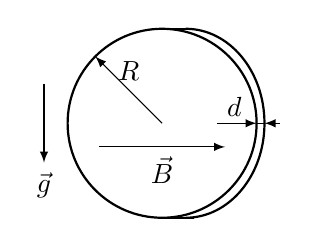
\begin{tikzpicture}
	\draw [thick] (0,0) circle (1.2);
	\draw [arrows={-latex}] (-1.5,0.5) -- (-1.5, -0.5) node [below] {$\vec{g}$};
	\draw [arrows={-latex}] (-0.8,-0.3) -- (0.8,-0.3) node [midway, below] {$\vec{B}$};
	\draw [thick] (0.3,-1.2) arc (-90:90:1.0 and 1.2);
	\draw [thick] (0,-1.2) -- (0.4,-1.2);
	\draw [thick] (0,1.2) -- (0.4,1.2);
	\draw [arrows={-latex}] (0.7,0) -- (1.2,0) node [left=8pt, above=-1pt] {$d$};
	\draw [arrows={-latex}] (1.5,0) -- (1.3,0);
	\draw (1.2,0) -- (1.3,0);
	\draw [arrows={-latex}] (0,0) -- (-0.8485,0.8485) node [midway, above=] {$R$};
\end{tikzpicture}
\end{document}